\section{Spécifications Techniques}


\subsection{Évaluation comparative des technologies.}
\begin{frame}{Benchmark Backend}
    \begin{figure}[H]
        \centering
        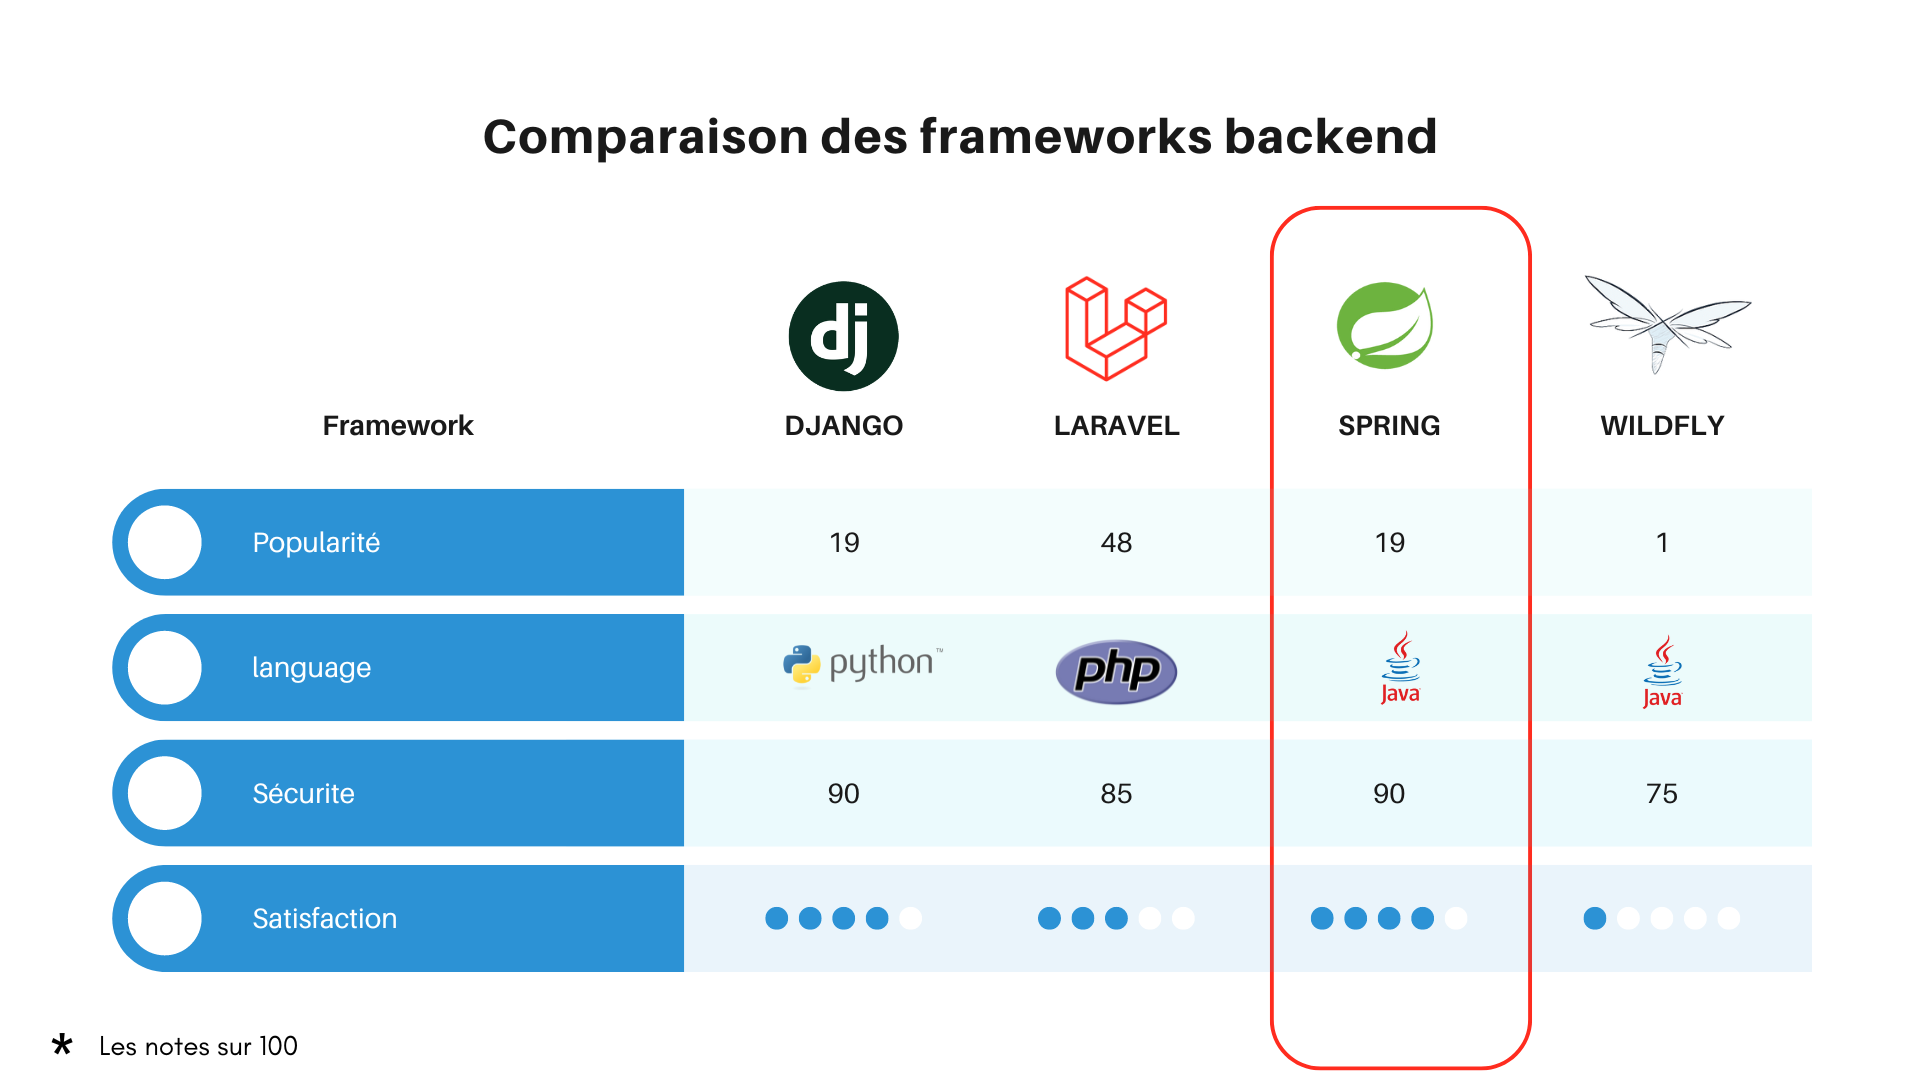
\includegraphics[height=5cm]{assets/images/benchmark.png}
    \end{figure}
\end{frame}

\begin{frame}{Benchmark Fronted}
    \begin{figure}[H]
        \centering
        
\includegraphics[height=5cm]{assets/images/bench-next.jpg}
    \end{figure}
\end{frame}

\begin{frame}{Benchmark model IA}
    \begin{figure}[H]
        \centering
        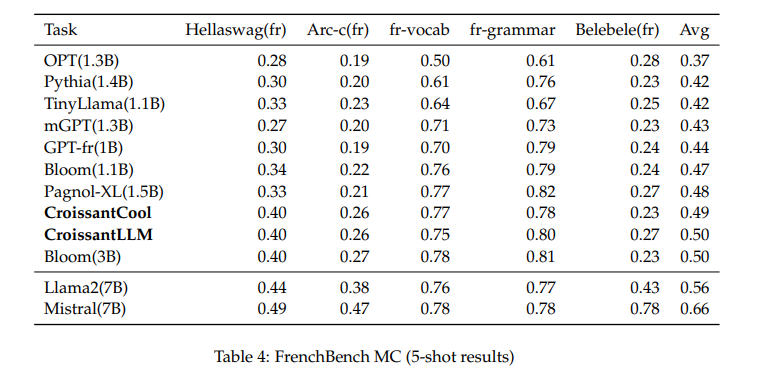
\includegraphics[height=6cm]{assets/images/ia_benchmark.png}
    \end{figure}
\end{frame}

\subsection{Technologies Sélectionnées}
\begin{frame}{Technologies choisies pour les services}
    \begin{figure}[H]
        \centering
        \begin{minipage}{0.32\textwidth}
            \centering
            
\includegraphics[height=3cm]{assets/images/next.png}
        \end{minipage}%
        \hspace{0.03\textwidth}
        \begin{minipage}{0.32\textwidth}
            \centering
            
\includegraphics[height=3cm]{assets/images/spring.png}
        \end{minipage}%
        \hspace{0.03\textwidth}
        \begin{minipage}{0.32\textwidth}
            \centering
            
\includegraphics[height=3cm]{assets/images/keycloak.png}
        \end{minipage}

    \end{figure}
\end{frame}



\begin{frame}{Technologies choisies pour IA}
    \begin{figure}[H]
        \centering

        \begin{minipage}{0.5\textwidth}
            \centering
            
\includegraphics[height=2cm]{assets/images/tinyllama.png}
        \end{minipage}
        \hspace{0.1\textwidth}
        \begin{minipage}{0.5\textwidth}
            \centering
            
\includegraphics[height=2cm]{assets/images/langchain.jpeg}
        \end{minipage}
        \hspace{0.1\textwidth}
        \begin{minipage}{0.5\textwidth}
            \centering
            
\includegraphics[height=2cm]{assets/images/mongo.png}
        \end{minipage}
    \end{figure}
\end{frame}

\subsection{Communication entre services}
\begin{frame}{Communication entre services}
    \begin{figure}[H]
        \centering
        
\includegraphics[height=2cm]{assets/images/rest.png}
        \hspace{0.1\textwidth}
        
\includegraphics[height=2cm]{assets/images/kafka.png}
    \end{figure}
\end{frame}

\subsection{Conclusion}
\begin{frame}{Conclusion}

    Cette étude technique détaille l\'architecture des microservices, les technologies utilisées, et les interactions entre les services, garantissant une application modulaire, sécurisée, et scalable avec Keycloak pour la gestion des identités et des accès. Les choix de conception visent à assurer une expérience utilisateur optimale tout en garantissant performance et sécurité.
\end{frame}
